\documentclass{article}

\usepackage[utf8]{inputenc}
\usepackage{amsmath}
\usepackage{amsfonts}
\usepackage{amssymb}
\usepackage{graphicx}
\usepackage[table,xcdraw]{xcolor}
\usepackage[hidelinks]{hyperref}
\usepackage{fontawesome5}
\usepackage{longtable}


\graphicspath{ {./images/} }

\renewcommand{\contentsname}{Indice}

\makeatletter
\newcommand*{\rom}[1]{\expandafter\@slowromancap\romannumeral #1@}
\makeatother

\usepackage[a4paper,top=2cm,bottom=2cm,left=2cm,right=2cm]{geometry}


\title{\textbf{\Huge Sviluppo Applicazione}}
\author{Edoardo Ghirardello, Giulio Cappelli, Elia Casotti \\ \\ Gruppo T42}
\date{2022}

\let\origthesubsection\thesubsection

\begin{document}

\maketitle

\clearpage
\tableofcontents
\clearpage

\section{Scopo del documento}
\begin{description}
    \item[] Nel documento corrente vengono riportate ulteriori e definitive informazioni riguardo allo sviluppo dell'applicazione Fen Festa.
        \\ Nello specifico, presenta tutti gli artefatti necessari per il login, la ricerca e la creazione degli eventi dell'applicazione. In partenza viene analizzato lo User-flow legato ad un utente registrato dell'applicazione, dopodiché vengono analizzate le API (tramite l'API Model) per la creazione, modifica e login di un profilo, le strutture dati, la visualizzazione, creazione e modifica di un evento necessari a Fen Festa.
    \item[] Per ogni API che è stata utilizzata, vengono presentate descrizione delle funzionalità, documentazione e test utilizzati
    \item[] In ultima istanza vengono fornite informazioni del Git Repository e, infine, il deployment dell'applicazione.
\end{description}
\clearpage
\section{User-Flows}
\begin{description}
    \item[] In questa sezione vengono riportati gli “user-flows” dell'utente registrato (che quindi può anche essere organizzatore o admin) della nostra applicazione.
    \item[] In \hyperref[img:1]{Figura 1} viene mostrato lo user-flow relativo alle azioni disponibili dall'homepage dagli utenti: visualizzazione, partecipazione e aggiunta preferiti degli eventi; in aggiunta anche la creazione evento se l'utente ha i permessi da organizzatore.
    \item[] L'utente può visualizzare gli eventi tramite mappa o calendario e aggiungerli ai preferiti, in entrambi i casi, una volta avvenuta la visualizzazione di questi ultimi. Lo schema utilizza la notazione “Pausa” quando l'azione non è disponibile e la notazione “Arrivo” quando viene raggiunta l'ultima azione disponibile per quel ramo.
    \item[] Viene, inoltre, presentata una legenda che descrive i simboli utilizzati, sempre in \hyperref[img:1]{Figura 1}.
    \item[] \label{img:1} \begin{center}
            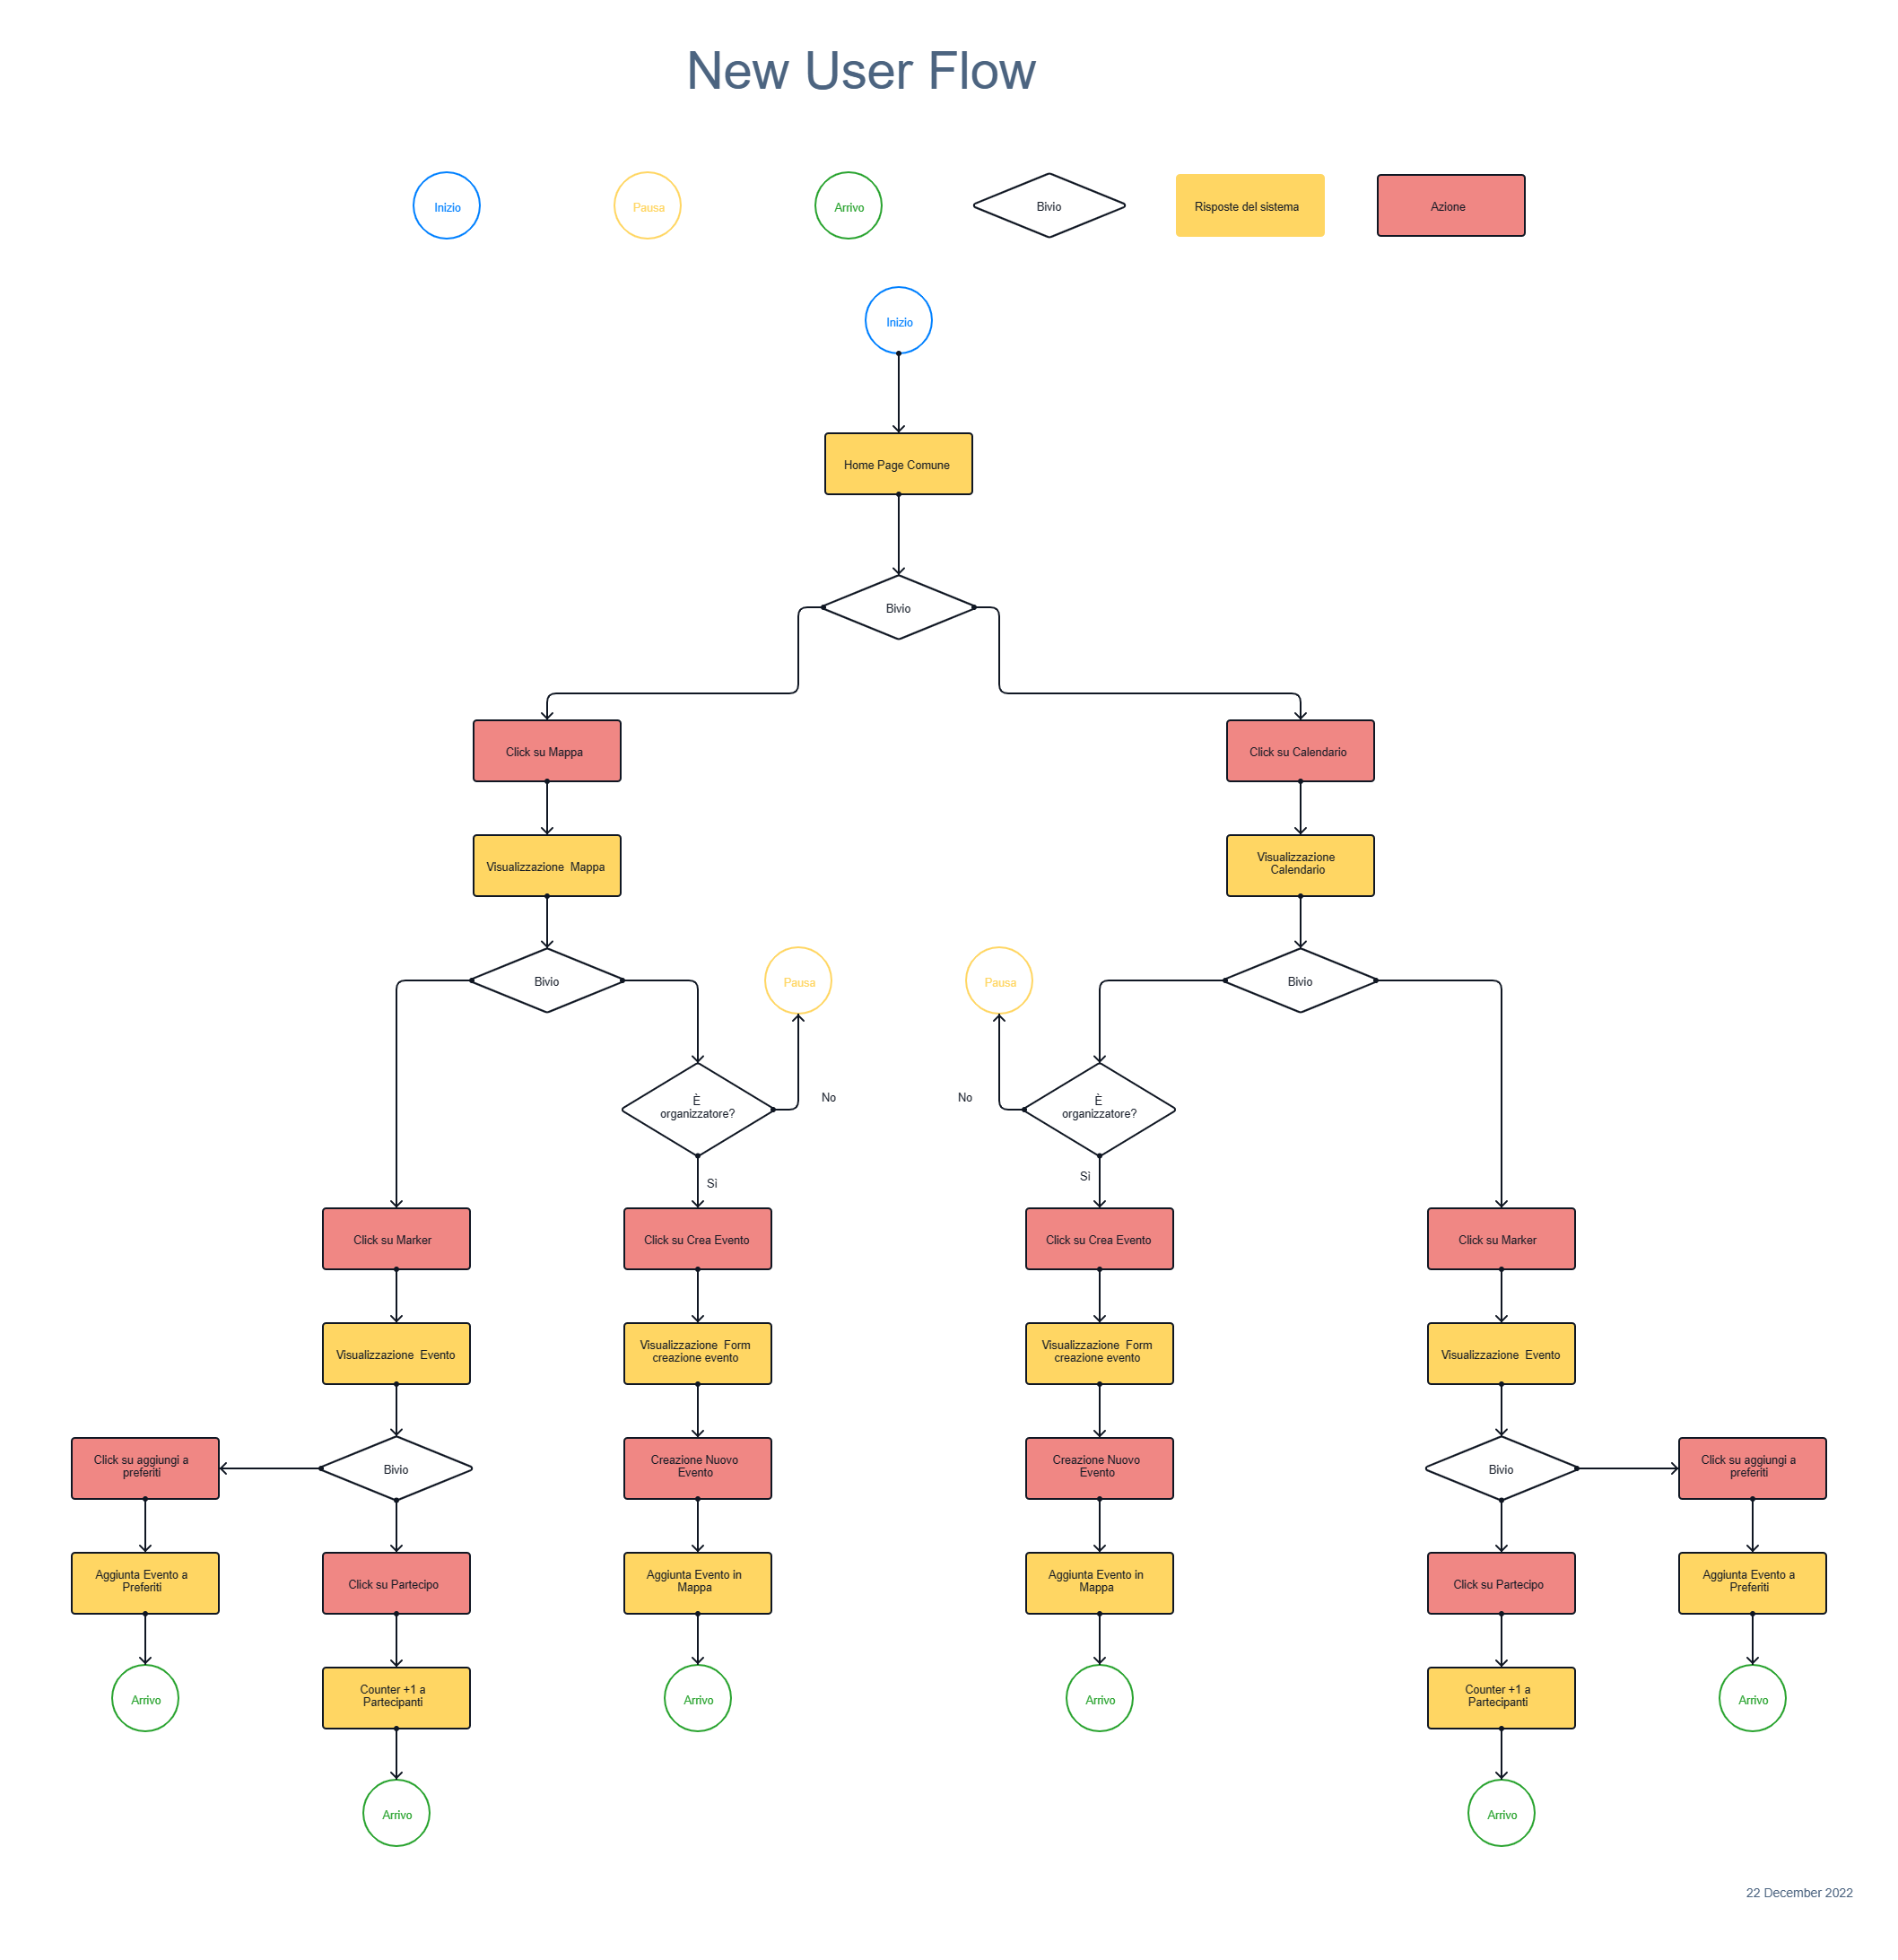
\includegraphics[scale=0.225]{User-Flow.png}
        \end{center}
\end{description}
\clearpage
\section{Application Implementation and Documentation}
\begin{description}
    \item[] Nei precedenti documenti sono stati identificati tutti i requisiti funzionali e non funzionali
        dell'applicazione. Nella sezione precedente son state descritte le features che servono ad un Utente nel
        suo flusso applicativo.
    \item[] Nella seguente sezione vengono analizzati i software e i tools di sviluppo di Fen Festa. L'applicazione è
        stata sviluppata utilizzando React (front-end) e NodeJS (back-end). Per la gestione dei dati è stato
        utilizzato MongoDB.
\end{description}
\subsection{Project Structure}
\begin{description}
    \item[]
\end{description}
\clearpage
\subsection{Project Dependencies}
\begin{description}
    \item[] Sono stati utilizzati e aggiunti al file \textbf{package.json} e seguenti moduli Node:
        \begin{itemize}
            \item bcrypt
            \item dotenv
            \item express
            \item jsonwebtoken
            \item mongoose
            \item multer
            \item nodemailer
            \item swagger-jsdoc
            \item swagger-ui-express
        \end{itemize}
\end{description}
\clearpage
\subsection{Project Data}
\begin{description}
    \item[] Per la gestione dati dell'applicazione viene usato un database.
\end{description}
\clearpage
\subsection{Project APIs}
\begin{description}
    \item[]
\end{description}
\clearpage
\section{API Documentation}
\begin{description}
    \item[] Le API Locali, descritte nella sezione precedente, fornite dall'applicazione FenFesta sono state documentate utilizzando il modulo NodeJS chiamato Swagger UI Express.
    \item[] Così facendo, aprendo la pagina designata, il reperimento della documentazione relativa alle suddette API è facilmente consultabile da qualunque persona.
    \item[] Per poter generare l'endpoint dedicato alla presentazione delle API è stato utilizzato Swagger UI in quanto crea una pagina web dalle definizioni delle specifiche OpenAPI.
    \item[] Di seguito viene mostrata la pagina web relativa alla documentazione che presenta le 5 API utilizzabili dall'utente generico per la visualizzazione degli eventi, partecipazione e salvataggio dell'evento con avviso.
    \item[] L'endpoint da invocare per raggiungere la seguente documentazione è: \url{http://localhost:3300/api-docs}
\end{description}
\clearpage
\section{Front-End Implementation}
\begin{description}
    \item[] Il Font-End fornisce una visualizzazione grafica rispetto alle funzioni di:
        \begin{itemize}
            \item Creazione dell'Account
            \item Mappa Eventi
            \item Calendario Eventi
            \item Creazione di un Nuovo Evento
            \item Visualizzazione Evento
        \end{itemize}
    \item[] In particolare, tali funzioni sono suddivise nelle 5 schermate rinominate:
        \begin{itemize}
            \item Creazione Account
            \item Mappa
            \item Calendario
            \item Creazione
            \item Visualizza Evento
        \end{itemize}
\end{description}
\clearpage
\subsection{Mappa Eventi}
\begin{description}
    \item[] \begin{center}
            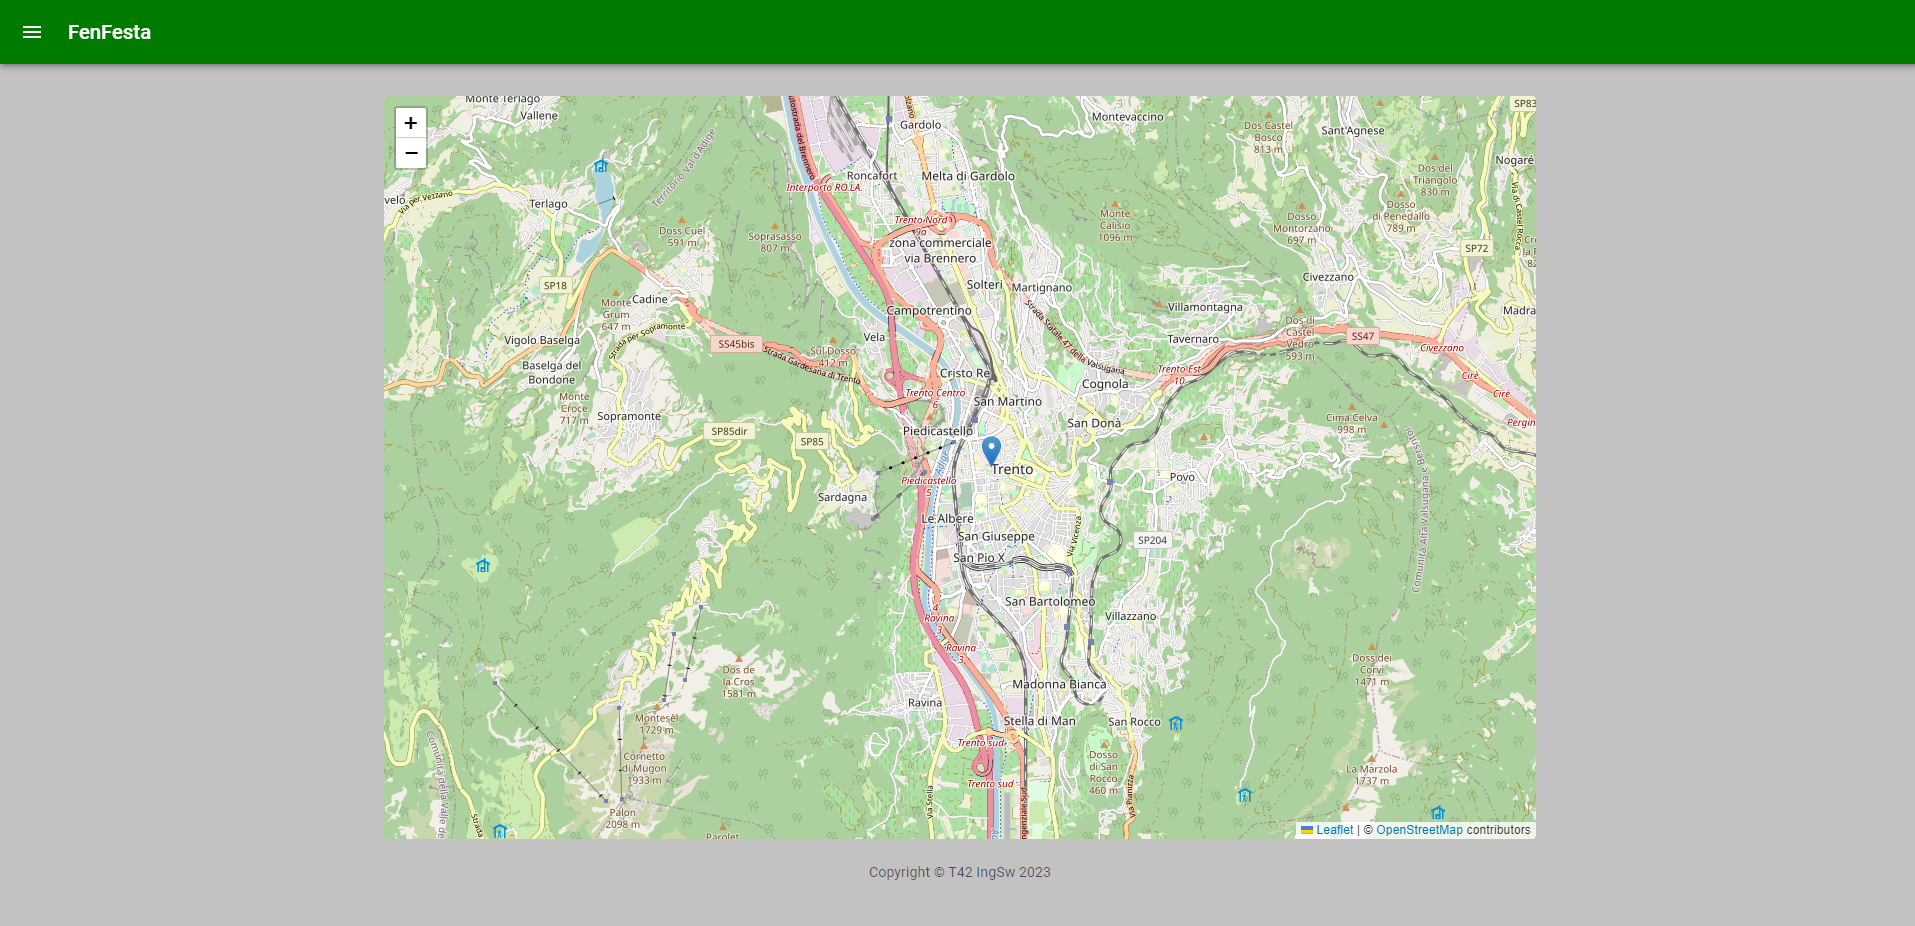
\includegraphics[scale=0.3]{Mappa_Eventi.png}
        \end{center}
    \item[] Nella sezione Mappa si può visualizzare una cartina interagibile, inserita grazie alle API di OpenStreetMap, nella quale sono posizionati dei marker che determinano la presenza di un Evento in quel punto. \\ Cliccandoci sopra si aprirà la sezione “Visualizza Evento”.
\end{description}
\subsection{Elenco Eventi}
\begin{description}
    \item[] \begin{center}
            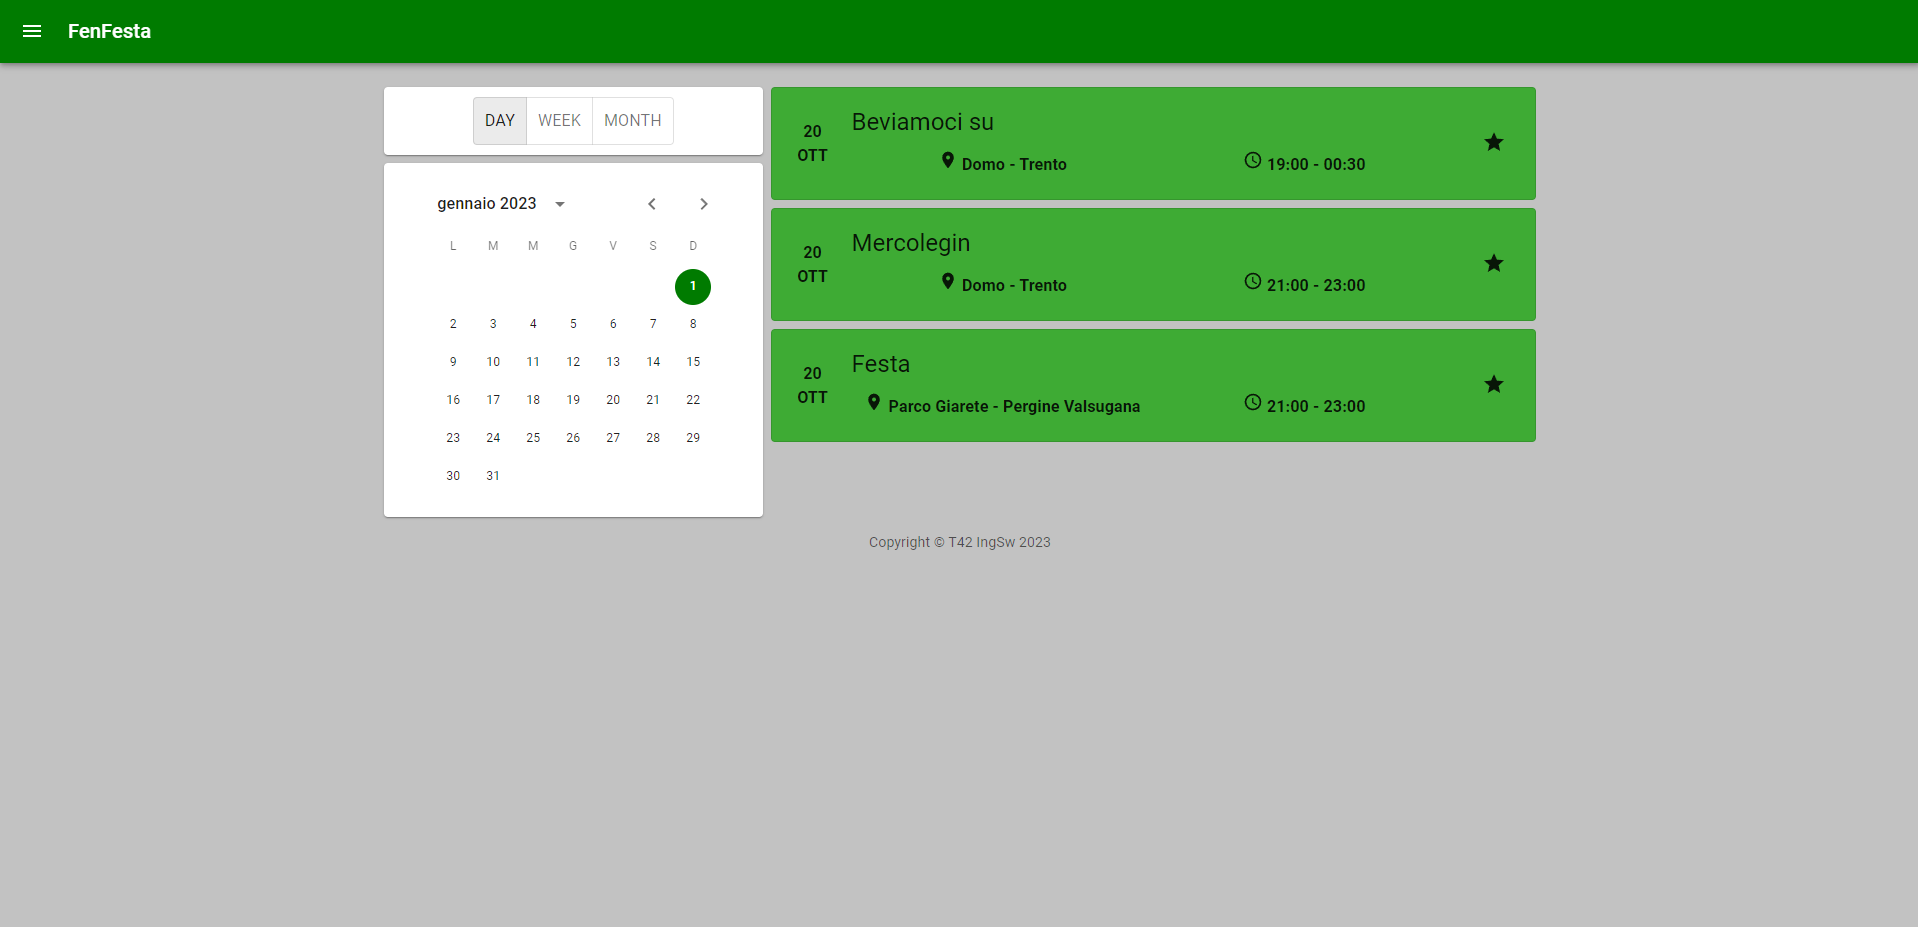
\includegraphics[scale=0.3]{Elenco_Eventi.png}
        \end{center}
    \item[] Nella schermata Calendario Eventi è disponibile un calendario con i giorni dell'anno ad accompagnare una lista di eventi disponibili giornalieri, settimanali o mensili
    \item[] Come nella Mappa, anche in questa schermata selezionando l'evento a cui si è interessati si aprirà la schermata di visualizzazione evento.
    \item[] Per selezionare l'Elenco o la Mappa è presente un menù laterale dove si può selezionare una delle due schermate
\end{description}
\clearpage
\subsection{Visualizza Evento}
\begin{description}
    \item[] \begin{center}
            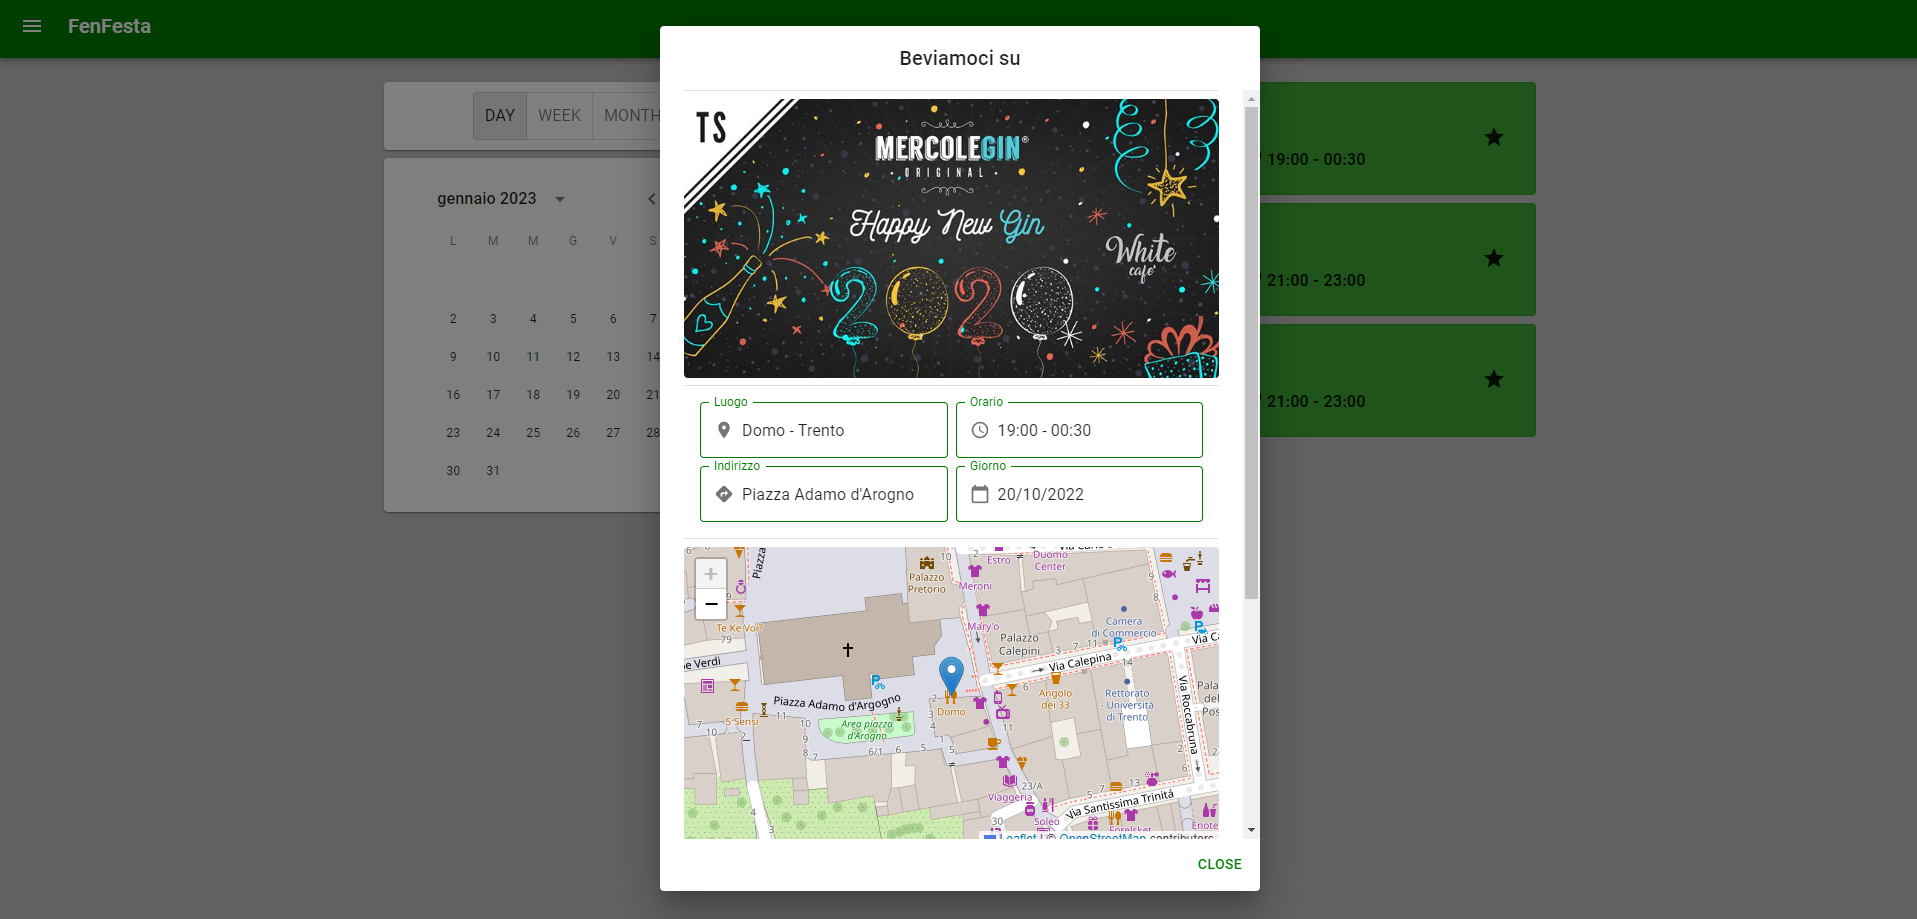
\includegraphics[scale=0.3]{Visualizza_Evento.png}
        \end{center}
    \item[] In questa sezione sono contenute tutte le informazioni relative all'evento (prese dal database). Sono presenti: immagine dell'evento, nome, data, orario, luogo, descrizione, tags, numero partecipanti, tasto “Partecipo”, tasto “Salva Evento”.
    \item[] Tramite il primo tasto viene aggiunta una persona al counter dei partecipanti; con la pressione del secondo, invece, si viene notificati della prossimità dell'evento tramite mail, il giorno stesso dell'evento.
    \item[] Questa schermata viene visualizzata sia quando si seleziona un evento dall'Elenco sia selezionando l'evento attraverso la Mappa
\end{description}
\subsection{Creazione Evento}
\begin{description}
    \item[] \begin{center}
            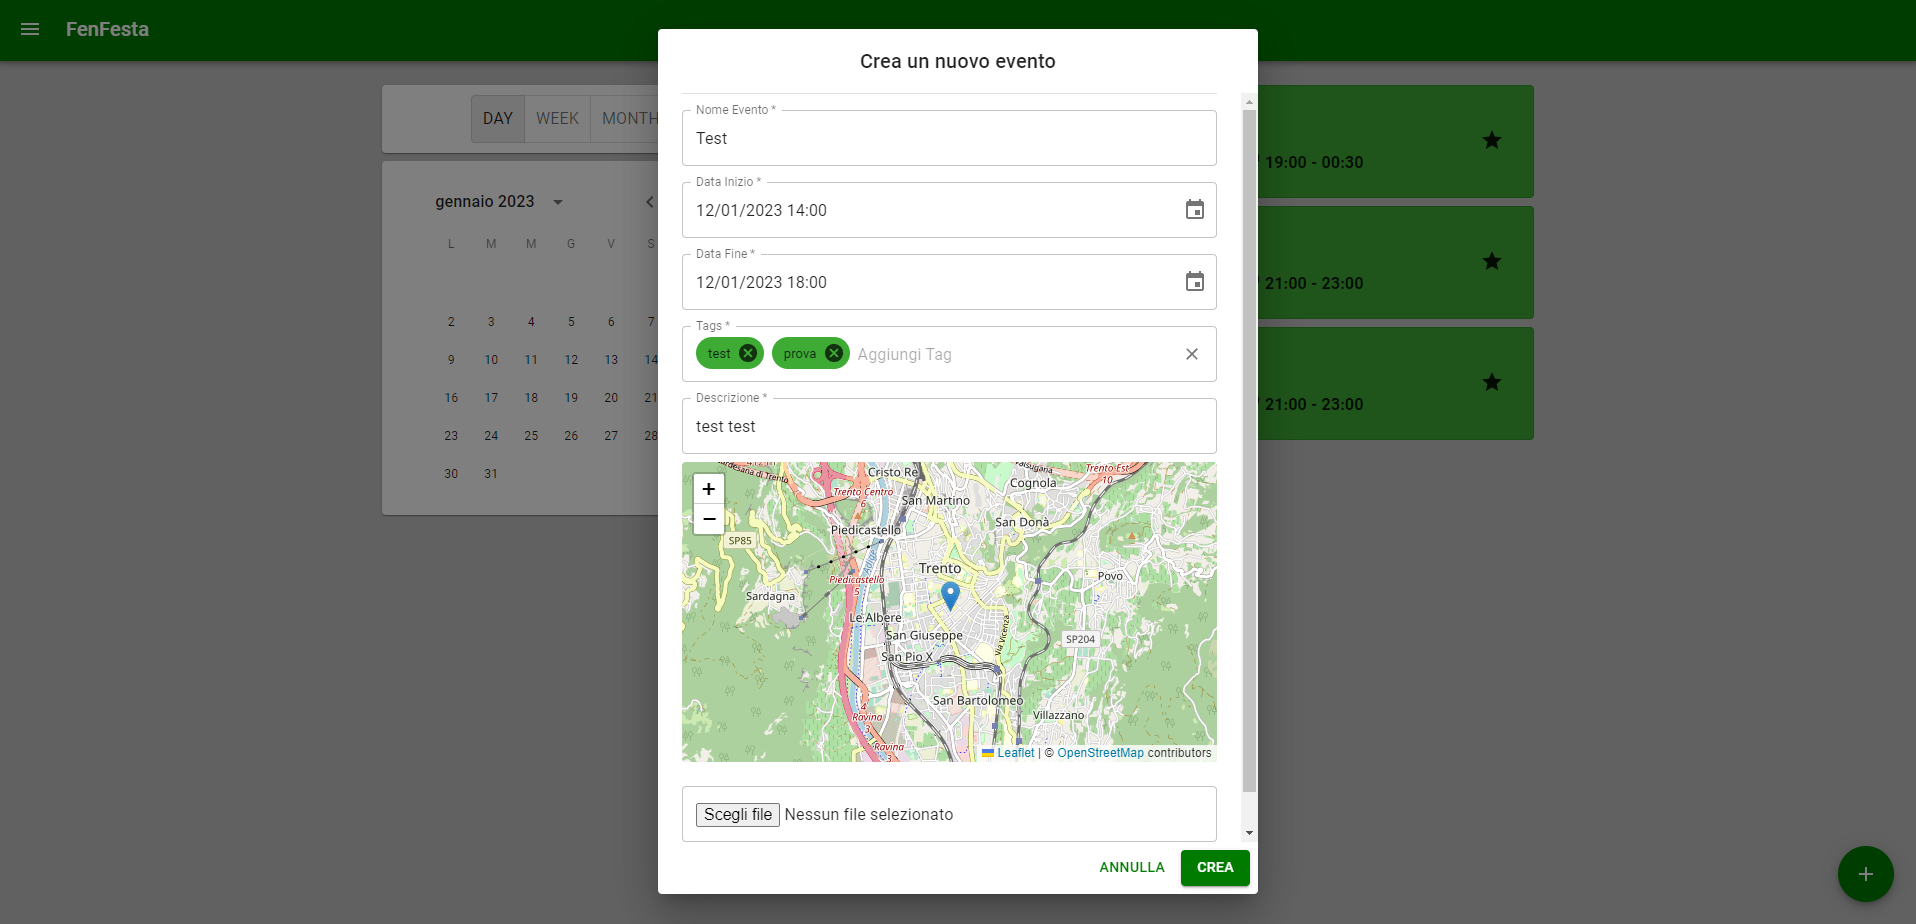
\includegraphics[scale=0.3]{Creazione_Evento.png}
        \end{center}
    \item[] Mediante la pressione di un tasto con l'icona di un + in una delle due schermate: Elenco o Mappa Eventi, e solo se si ha un account organizzatore, viene aperta la schermata di creazione Evento. È presente un form per l'inserimento di tutte le informazioni necessarie per la creazione, quali: immagine dell'evento, nome, data e orario, luogo, descrizione, tags.
    \item[] Premendo il tasto “Crea”, l'evento verrà registrato nel database e inserito nell'elenco eventi visualizzato tramite Mappa o Calendario
\end{description}
\clearpage
\section{GitHub Repository and Deployment Info}
\begin{description}
    \item[] Il progetto FenFesta è disponibile al seguente link: \url{https://github.com/T42CaCaGhi-Project}
    \item[] Per esegiure il front-end è necessario clonare la repository e successivamente utlizzare i comandi:
        \begin{enumerate}
            \item \texttt{npm install} per installare le varie dipendenze
            \item \texttt{npm start} per far partire il front-end
        \end{enumerate}
    \item[] Per esegiure il back-end è necessario clonare la repository e successivamente utlizzare i comandi:
        \begin{enumerate}
            \item \texttt{npm install} per installare le varie dipendenze
            \item \texttt{npm start} per far partire il back-end
        \end{enumerate}
    \item[] Per esegiure i test sulle API è necessario clonare la repository del back-end e successivamente utlizzare i comandi:
        \begin{enumerate}
            \item \texttt{npm install} per installare le varie dipendenze
            \item \texttt{npm run test} per far partire i test sulle API
        \end{enumerate}
\end{description}
\clearpage
\section{Testing}
\begin{description}
    \item[]
\end{description}
\end{document}